\documentclass[a4paper,12pt,oneside,final]{extarticle}
\usepackage[top=2cm, bottom=2cm, left=3cm, right=1cm]{geometry}
\usepackage{scrextend}

\usepackage[T2A,T1]{fontenc}
\usepackage[ukrainian,russian,english]{babel}
\usepackage{tempora}
\usepackage{fontspec}
\setmainfont{tempora}

\frenchspacing

% Lists
\usepackage{enumitem}
\renewcommand\labelitemi{--}
\renewcommand\labelenumi{\arabic*}
\setlist[description]{noitemsep,style=multiline,leftmargin=2.5cm}
\setlist[itemize]{noitemsep, topsep=0pt}
\setlist[enumerate]{noitemsep, topsep=0pt}

\usepackage{titlesec}
\newcommand{\sectionbreak}{\clearpage}

\usepackage{hyperref} % make refs clickable
\usepackage{float}
\usepackage{pgfplots}
\usepackage{graphicx}
\usepackage{multirow}
\usepackage{amssymb,amsfonts,amsmath,amsthm}
\usepackage{csquotes}
\usepackage{xstring}

\numberwithin{equation}{section}

\usepackage{listings}
\lstset{basicstyle=\footnotesize\ttfamily,breaklines=true}
\lstset{language=Matlab}

\begin{document}
\Russian
\title{Основы управление развитием организации}
\maketitle
\tableofcontents

%
% section 1
%
\section{Модуль I}
\subsection{Понятие и сущность управления}

\subsection{Управление и менеджеры}

\subsection{Развитие теории и практики управления. Современная система взглядов на управление}

\subsection{Определение <<организационная система>>. Организационные системы как системы междисциплинарной природы}

\subsection{Внутренняя и внешняя среда организационной системы}
Внутренняя среда организационной системы --- это ее организационное строение и ситуационные факторы внутри нее (внутренние переменные).
К основным переменным относятся: структура, цели, задачи, технологии и люди.

Производство --- это средства и предметы труда, а также трудовые ресурсы.

Внешняя среда организации --- это силы внешние по отношению к организации, которые действуют на ее результативность. 
Факторы, оказывающие немедленное воздействие или влияние на организацию --- это среда прямого воздействия, а все другие --- косвенного.

Выделяют 4 (четыре) основных свойства внешней среды: 
\begin{itemize}
	\item взаимосвязанность факторов внешней среды (уровень силы, с которой изменение одного фактора воздействует на другие); 
	\item сложность внешней среды (количество факторов и уровень вариативности); 
	\item подвижность среды (скорость, с которой могут меняться факторы); 
	\item неопределенность среды (является функцией количества информации, которой располагает организация по поводу конкретного факторы, а также функция уверенности в этой информации). 
\end{itemize}

\subsection{Задачи управления организационными системами}

\subsection{Понятие принципа и роль в управлении организационной системой}

\subsection{Содержание основных принципов управления}

\subsection{Цели организационных систем и их классификация}

\subsection{Понятие об управленческом цикле}

\subsection{Характеристика функций управления}

\subsection{Понятие коммуникаций и их роль в системе управления}

\subsection{Процесс коммуникаций: модель, основные этапы и элементы}

\subsection{Понятие и основные элементы процесса управления}

\subsection{Управленческое решение. Этапы и процедуры процесса принятия решений}

\subsection{Необходимость моделирования. Обзор моделей науки управления}

\subsection{Общенаучные методы}

\subsection{Конкретные или специфические методы управления}

\subsection{Сущность и смысл контроля}

\subsection{Процесс контроля}

\subsection{Характеристики эффективного контроля}

%
% section 2
%
\section{Модуль II}
\subsection{Концепция управления персоналом}

\subsection{Принципы управления персоналом}

\subsection{Методы построения системы управления персоналом}

\subsection{Методы управления персоналом}

\subsection{Источники организации найма персонала}

\subsection{Требования к кандидатам на замещение вакантной должности}

\subsection{Организация процесса отбора претендентов на вакантную должность}

\subsection{Сущность и виды профориентации и адаптации персонала}

\subsection{Опыт профориентации и адаптации персонала}

\subsection{Организация управления профориентацией и адаптацией персонала}

\subsection{Изучение состояния работы по профориентации и адаптации персонала}

\subsection{Группы и их значимость}

\subsection{Управление неформальной организацией }

\subsection{Повышение эффективности работы групп. Факторы, влияющие на эффективность деятельности групп и организации}

\subsection{Власть, влияние}

\subsection{Убеждение и участие}

\subsection{Основы лидерства}

\subsection{Традиционные концепции лидерства}

\subsection{Концепции ситуационного лидерства}

\subsection{Новое в теориях лидерства}

\subsection{Природа конфликта и стресса}

\subsection{Управление конфликтной ситуацией}

\subsection{Управление изменениями}

\subsection{Сущность, функции и элементы маркетинга}
Маркетинг --- это комплексная система организации производства и сбыта, ориентированная на возможное более полное удовлетворение быстро меняющихся и все более разнообразных потребностей потребителей посредством рынка и получение на этой основе устойчивой прибыли и конкурентных преимуществ.

Выделяют 3 (три) подхода к определению сущности маркетинга:
\begin{itemize}
	\item как самостоятельный вид производственной деятельности;
	\item как функция управления;
	\item как современное видение философии бизнеса.
\end{itemize}

Концепция маркетинга --- это философия управления, которая способствует получению товара производителями прибыли посредством удовлетворения потребностей потребителей.

% http://www.grandars.ru/student/marketing/funkcii-marketinga.html
Главные функции маркетинга:
\begin{itemize}
	\item аналитическая функция;
	\item продуктово-производственная функция;
	\item сбытовая функция (функция продаж);
	\item функция управления и контроля.
\end{itemize}

Комплекс маркетинга --- совокупность управляемых элементов маркетинговой деятельности организации, манипулируя которыми она старается наилучшим образом удовлетворить потребности целевых рынков.
% https://ru.wikipedia.org/wiki/%D0%A2%D0%B5%D0%BE%D1%80%D0%B8%D1%8F_4P
Теория 4P \textit{(маркетинг-микс)} — маркетинговая теория, основанная на четырёх основных <<координатах>> маркетингового планирования:
\begin{description}
	\item[Product] Товар или услуга, ассортимент, качество, свойства товара, дизайн и эргономика.
	\item[Price] Цена, наценки, скидки.
	\item[Promotion] Продвижение, реклама, пиар, стимулирование сбыта.
	\item[Place] Месторасположения торговой точки, каналы распределения, персонал продавца.
\end{description}

\subsection{Задачи, виды и структура маркетинговых исследований}
Маркетинговое исследование --- это систематический поиск, сбор, анализ и представление данных и сведений, относящихся к конкретной рыночной ситуации, с которой пришлось столкнуться предприятию. 
Маркетинговое исследование можно также определить как систематический сбор, учет и анализ данных по маркетингу и маркетинговым проблемам в целях совершенствования качества процедур принятия решений и контроля в маркетинговой среде. 
Имеется целый ряд аналогичных и иных определений маркетинговых исследований.

Основные цели маркетингового исследования:
\begin{itemize}
	\item уменьшить неопределенность и минимизировать риск в процессе принятия управленческих решений;
	\item следить за процессом реализации маркетинговых задач.
\end{itemize}

Глобальные цели маркетингового исследования --- это информационное обеспечение маркетинга, то есть сбор необходимой информации и аналитическое обеспечение, заключающееся в использовании математических моделей для анализа данных и получения с их помощью прогнозов и возможности принятия оптимальных решений.

% http://works.doklad.ru/view/hARiKdLaWJM.html
Задачи маркетинговых исследований могут быть самыми разнообразными и диктоваться потребностями разработки стратегии маркетинга, формирование ценовой, товарной, коммуникационной, сбытовой политики и другими аспектами управления маркетингом на предприятии. 
Наиболее типичные решаемые задачи маркетинговых исследований:
\begin{itemize}
	\item изучение характеристик рынка;
	\item замеры потенциальных возможностей рынка;
	\item анализ распределения долей рынка между фирмами;
	\item анализ сбыта;
	\item изучение тенденций деловой активности;
	\item изучение товаров конкурентов;
	\item краткосрочное прогнозирование;
	\item изучение реакции на новый товар и его потенциала;
	\item долгосрочное прогнозирование;
	\item изучение политики цен.
\end{itemize}

\begin{figure}[h]
	\centering
	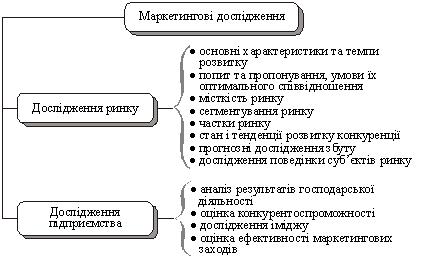
\includegraphics{management-figures/marketing_structure}
	\caption{Структура маркетинговых исследований}
\end{figure}

Типы маркетинговых исследований:
\begin{enumerate}
	\item Разведочные или поисковые, предшествующие разработке программы основного исследования. 
	Предпринимаются для сбора предварительной информации, освещающие проблемы, позволяет выдвинуть гипотезы.
	\item Описательные \textit{(дескриптивные)}. 
	Имеющие целью констатацию реальных фактов, событий, показателей, полученных в результате сбора информации. 
	\item Экспериментальные. 
	Проводится с целью проверки выдвинутой гипотезы.
	\item Аналитические. 
	Проводимое для выявления и моделирования связи и деятельности фирмы с факторами окружающей среды. 
\end{enumerate}

\subsection{Маркетинговое сегментирование рынка}
Сегментирование рынка --- это процесс разделения рынка на отдельные части --- сегменты, отличающиеся друг от друга разными возможностями сбыта.

Сегмент рынка --- это особым образом выделенная часть рынка, группы потребителей или предприятий, обладающих определенными общими признаками. 
Может быть осуществлено по множеству критериев --- мерилам оценки обоснованности выбора сегмента рынка. 
Принцип сегментирования --- показатель выделения данного сегмента рынка. 

\begin{figure}[h]
	% http://powerbranding.ru/segmentirovanie/osnovy/
	\centering
	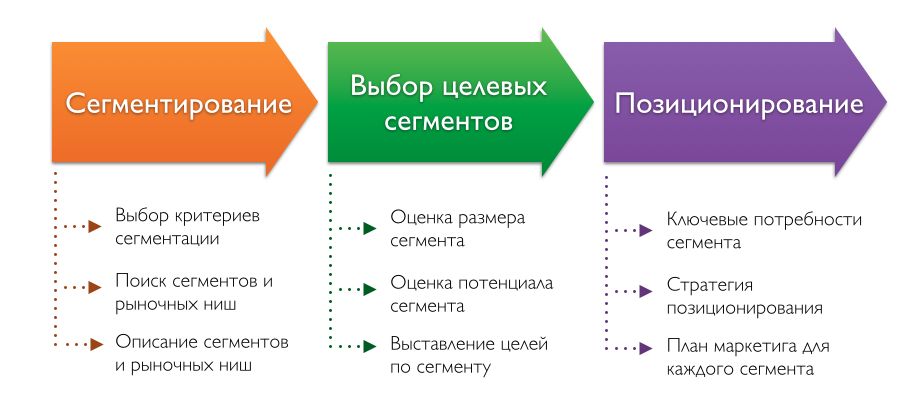
\includegraphics[width=\textwidth]{management-figures/marketing_segmentation_process}
	\caption{Схема сегментации рынка}
\end{figure}

Могут быть использованы следующие критерии:
\begin{enumerate}
	\item Различия между потребителями позволяющее объединить их в один сегмент.
	\item Сходство, формирующие устойчивость.
	\item Наличие показателей, позволяющих измерить характеристики и требования потребителей, определить емкость рынка.
	\item Возможность выстоять в конкурентной борьбе.
	\item Достаточность объема продаж.
	\item Доступность сегмента для предприятия.
\end{enumerate}

Существует три варианта охвата рынка:
\begin{itemize}
	\item недифференцированный маркетинг;
	\item дифференцированный маркетинг;
	\item концентрированный маркетинг.
\end{itemize}

\subsection{Цель и суть товарной политики}
Товарная политика --- это совокупность решений, касающихся формирования эффективной рыночно-ориентированной производственной программы предприятия.

Товарная политика ­­--- область целенаправленных действий по отдельным предложенным для использования товарам и услугам (вид, количество, свойство и т.д.), а также по совокупности отдельных продуктов (ширина, глубина, структура ассортимента).

Цель товарной политики --- добиться сбалансированного товарного ассортимента и конкурентоспособности каждого отдельного продукта, а так же:
\begin{itemize}
		\item обеспечение прибыли;
		\item увеличение товарооборота;
		\item увеличение доли рынка;
		\item снижение расходов на производство и маркетинг;
		\item повышение имиджа;
		\item рассеивание риска.
\end{itemize}

Задачи товарной политики --- принятие решений в области предлагаемых предприятием товаров, касающихся самих продуктов, их присутствия на рынке, а также связанных с этим решений по производственной программе.

\subsection{Использование средств стимулирования сбыта}

\subsection{Ценовая политика в маркетинговой деятельности. Методы расчета и установления цены}

\end{document}